\section{Discussion}

This section discusses the transition from project \emph{manager} to project \emph{leader} and how it may be handled.

\subsection{Need for leaders, not controllers}

Perhaps the most important finding in the literature is that agile projects do not \emph{need} a project manager in the traditional sense. This stems from the fact that agile projects heavily rely on teams to be self-organising and self-managing. These teams require to be coached and led – not commanded and controlled. One example of this is \autocite{yi:managerasscrummaster}, where the transition to self-managing teams involved eliminating most project managers and replacing the process with a Product Owner-centered mode of operation.

Furthermore, this leader must be responsible for removing impediments for the team. In Scrum, for example, the Daily Scrum (also known as Daily Standup or Morning Meeting) is designed to uncover impediments the team has encountered as soon as possible – but the project leader (Scrum Master) must take responsibility to remove these impediments \autocite{schwaber:scrum}.

\subsection{Several strategies to choose from}

Another very important issue is raised by \autocite{fernandez:agilevstraditional}: projects are different, and the same person may need to lead several projects within the same organisation under different circumstances. This means that agile is not the correct approach. In their article, they present the following figure to aid identification of the best strategy based on complexity and uncertainty:

\begin{figure}[H]
    \label{fig:projectcharacteristicsquadrants}
    \centerline{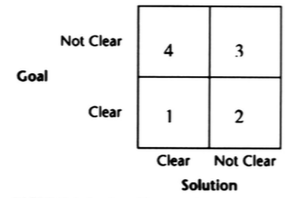
\includegraphics[scale=0.5]{project-characteristics-quadrants}}
    \caption{Project characterstics quadrants}
\end{figure}

They also present the following figure outlining five main strategies for the project based on which quadrant it fits into.

\begin{figure}[H]
    \label{fig:projectstrategies}
    \centerline{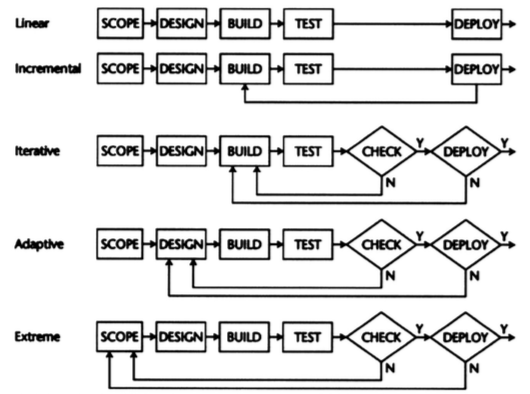
\includegraphics[scale=0.55]{project-strategies}}
    \caption{Project strategies}
\end{figure}

The main characteristics of the linear strategy (often referred to as a waterfall because of its incapability of revisiting previous phases) are that scope and design is decided before any building takes place. Testing takes place \emph{after} building is complete, and deployment follows testing. The incremental strategy releases the product in increments, but does not respond to changes in scope or design. The iterative, adaptive, and extreme strategies all share the basic concept that work is completed in increments and guided by a the owner of the final product, but differ in how much of the process is repeated in each iteration. Please refer to \autocite{fernandez:agilevstraditional} for an more in-depth description of each strategy.

They argue that a project that fits into quadrant 1 of Figure \ref{fig:projectcharacteristicsquadrants} is a good fit for the \emph{linear} or \emph{incremental} strategy because the both end goal (scope) and solution are clear from the very start of the project. If all that is required is implementing a known solution, then the iterative, adaptive, and extreme strategies all bring with them unnecessary overhead. The iterative strategy is the best choice if the project needs to be completed before the product is usable. The incremental strategy is better if the product is in a usable state before the project's completion.

However, if the end goal (scope) or solution is not known at the start of the project, iterating more of the development process means that the product is allowed to converge on a solution as new information is learned about the previously insecure factors. Additionally, business value is produced early in the project and incremented with each release.

Furthermore, there is a plethora of frameworks, methodologies, and techniques to choose from. Two of the most widely used tools in these categories are Kanban (conceived by Taiichi Ohno in an attempt to improve efficiency in Totyota and later adopted by the IT industry); Scrum \autocite{schwaber:scrum}; and Extreme Programming \autocite{beck:extreme}.

This all means that the transition from traditional project management to agile project management involves mastering the different available strategies. After the rise of agile strategies, methodologies, and frameworks, identifying and employing the best fit for the project is a critical skill in a project leader.

\subsection{Agile projects limit resources, not scope}

\citeauthor{cohn:agile} (\citeyear{cohn:agile}) equates the traditional view of a project as running a 10-kilometer race: the scope (goal, or finish line) is well-defined, and the solution is to run there as fast as possible. Agile projects, on the other hand, where the finish line is not certain by the start of the project, can be compared to a timed race where the goal is to get as far as possible within the allotted time. Following the analogy, the agile approach allows responding to unexpected bumps and unexpected turns in the road.

\autocite{fernandez:agilevstraditional} draw upon Wysocki's \emph{Effective Software Project Management} to contrast traditional and agile project managers, and use the same argument: while the traditional project manager wants to reduce risk and minimise time and money, the agile project manager focuses on delivering business value throughout the project – the timeline becomes secondary in agile projects.

In such a project, it is very important that everyone works with an agile \emph{mindset}: \citeauthor{fernandez:agilevstraditional} (\citeyear{fernandez:agilevstraditional}) conclude that simply following agile practises does not make the team agile; instead, they quote Cockburn (2005), who considers agile to be about \emph{attitude}: team agility is only a means to reach the best result within the given constraints. A project leader in an agile project, then, must ensure that everyone in the agile team properly \emph{understands} the agile principles and why they are important. It follows that inexperienced teams, and likely even experienced ones, require a role to call and lead meetings when necessary and ensures that the project is actually moving in the right direction; merely meeting with the product owner every few weeks does not imply that the project will be a success.

\subsection{Culture, coaching and leadership}

As discussed in the previous subsection, the team members must \emph{understand} why the agile aspect of the development process is helpful to the project as a whole: agile is about attitude, not about strictly following a set of rules. For this reason, it is important that the project utilises only tools that improve the development process. In his \citeyear{warstory} experience report on combining the agile framework Scrum \autocite{schwaber:scrum} and the more software-oriented Extreme Programming \autocite{beck:extreme} \citetitle{warstory}, \citeauthor{warstory} explains in detail how two tools can be utilised together for success. Of course, this tale only applied specifically to his case, but it shows that a project does not require \emph{many} tools to get the job done – only the \emph{correct} ones.

\citeauthor{warstory} also shows that following the tools strictly by the book (in this case \citeauthor{schwaber:scrum} (\citeyear{schwaber:scrum})) is not necessarily the best approach, and provides an implementation of Scrum and Extreme Programming that is successful to their domain. While not academic, these kinds of experience reports are valuable – although as mentioned in the literature review, many case studies of almost the same type already exist in the research body.

A final key point to make is that introducing agile principles and tools in a well-established organisation will result in dramatic cultural changes \autocite{nhn:agileadoption}. Again, the importance of the entire team understanding the importance of the practises comes up: especially in this period, the agile project leader must fully understand and be able to properly coach the team in their project's implementation of agile.

\subsection{Other factors: large-scale and distributed development}

As we can clearly see, there are many aspects of agile to consider when comparing the traditional project manager to the agile project leader. In addition to the issues relating to organisational culture and attitude, and selecting the strategy and tools that best fit the project at hand, there are (at least) two very important environmental challenges that many companies and projects face: projects of large scale, and projects that are distributed.

First, large-scale projects with many developers are a challenge: the optimum size of a Scrum team is recommended to be 7 plus minus 2 members \autocite{scrumprimer}. One solution to this problem can be to introduce new teams consisting of only the Scrum masters from related projects, to that all the project leader for each team will be able to distribute enough information about the other teams \autocite{lyon:scaling} \autocite{maranzato:megaframework}, although large-scale projects \emph{will} lose some agility \autocite{lyon:scaling}.

Finally, distributed projects may prove problematic to properly conduct. \citeauthor{suresshrini} (\citeyear{suresshrini}) has provided a transition model to counter this potential issue. \citeauthor{warstory} (\citeyear{warstory}) proposes to use digital tools in such a manner that the team can \emph{almost} communicate as though everyone were in the same room. The responsibility for facilitating these communication channels must be of the project leader – after all, not being able to communicate is an impediment for the development team.
